\chapter{Miscellanous tables, figures, UML Class diagrams}

\begin{table}[h]
\begin{center}
  \begin{tabular}{ c | *{16}{c}}
     & 00 & 01 & 02 & 03 & 04 & 05 & 06 & 07 & 08 & 09 & 0a & 0b & 0c & 0d & 0e & 0f \\ \hline
  00 & 63 & 7c & 77 & 7b & f2 & 6b & 6f & c5 & 30 & 01 & 67 & 2b & fe & d7 & ab & 76 \\ 
  10 & ca & 82 & c9 & 7d & fa & 59 & 47 & f0 & ad & d4 & a2 & af & 9c & a4 & 72 & c0 \\
  20 & b7 & fd & 93 & 26 & 36 & 3f & f7 & cc & 34 & a5 & e5 & f1 & 71 & d8 & 31 & 15 \\
  30 & 04 & c7 & 23 & c3 & 18 & 96 & 05 & 9a & 07 & 12 & 80 & e2 & eb & 27 & b2 & 75 \\
  40 & 09 & 83 & 2c & 1a & 1b & 6e & 5a & a0 & 52 & 3b & d6 & b3 & 29 & e3 & 2f & 84 \\
  50 & 53 & d1 & 00 & ed & 20 & fc & b1 & 5b & 6a & cb & be & 39 & 4a & 4c & 58 & cf \\
  60 & d0 & ef & aa & fb & 43 & 4d & 33 & 85 & 45 & f9 & 02 & 7f & 50 & 3c & 9f & a8 \\
  70 & 51 & a3 & 40 & 8f & 92 & 9d & 38 & f5 & bc & b6 & da & 21 & 10 & ff & f3 & d2 \\
  80 & cd & 0c & 13 & ec & 5f & 97 & 44 & 17 & c4 & a7 & 7e & 3d & 64 & 5d & 19 & 73 \\
  90 & 60 & 81 & 4f & dc & 22 & 2a & 90 & 88 & 46 & ee & b8 & 14 & de & 5e & 0b & db \\
  a0 & e0 & 32 & 3a & 0a & 49 & 06 & 24 & 5c & c2 & d3 & ac & 62 & 91 & 95 & e4 & 79 \\
  b0 & e7 & c8 & 37 & 6d & 8d & d5 & 4e & a9 & 6c & 56 & f4 & ea & 65 & 7a & ae & 08 \\
  c0 & ba & 78 & 25 & 2e & 1c & a6 & b4 & c6 & e8 & dd & 74 & 1f & 4b & bd & 8b & 8a \\
  d0 & 70 & 3e & b5 & 66 & 48 & 03 & f6 & 0e & 61 & 35 & 57 & b9 & 86 & c1 & 1d & 9e \\
  e0 & e1 & f8 & 98 & 11 & 69 & d9 & 8e & 94 & 9b & 1e & 87 & e9 & ce & 55 & 28 & df \\
  f0 & 8c & a1 & 89 & 0d & bf & e6 & 42 & 68 & 41 & 99 & 2d & 0f & b0 & 54 & bb & 16 \\
  \end{tabular}
  \caption{Gr{\o}stl S-box. For an input x, you do a logical AND of x with f0 and with 0f.
  The first value obtained is used for column location and second for row location. The
  row and column location is used to identify the cell that will be used for substitution.
  \cite{00019}}
  \label{table:Groestlsbox}
\end{center}
\end{table}

\begin{table}
\begin{center}
  \begin{tabular}{ c | *{8}{c} | }
      & 02 & 02 & 03 & 04 & 05 & 03 & 05 & 07 \\
      & 07 & 02 & 02 & 03 & 04 & 05 & 03 & 05 \\
      & 05 & 07 & 02 & 02 & 03 & 04 & 05 & 03 \\
  B = & 03 & 05 & 07 & 02 & 02 & 03 & 04 & 05 \\
      & 05 & 03 & 05 & 07 & 02 & 02 & 03 & 04 \\
      & 04 & 05 & 03 & 05 & 07 & 02 & 02 & 03 \\
      & 03 & 04 & 05 & 03 & 05 & 07 & 02 & 02 \\
      & 02 & 03 & 04 & 05 & 03 & 05 & 07 & 02 \\
  \end{tabular}
  \caption{Mix bytes matrix used in Gr{\o}stl permutation \cite{00019}.}
  \label{table:GroestlMixBytesMatrix}
\end{center}
\end{table}

\begin{figure}
  \begin{center}
    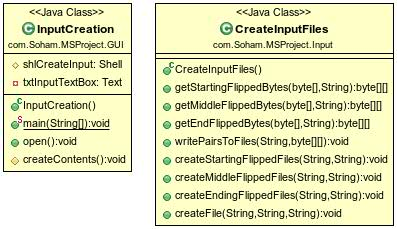
\includegraphics[width=4in]{Input.jpg}
  \end{center}
  \caption{Class diagram of the input creation.}
  \label{fig:UMLInputCreation}
\end{figure}

\begin{figure}
  \begin{center}
    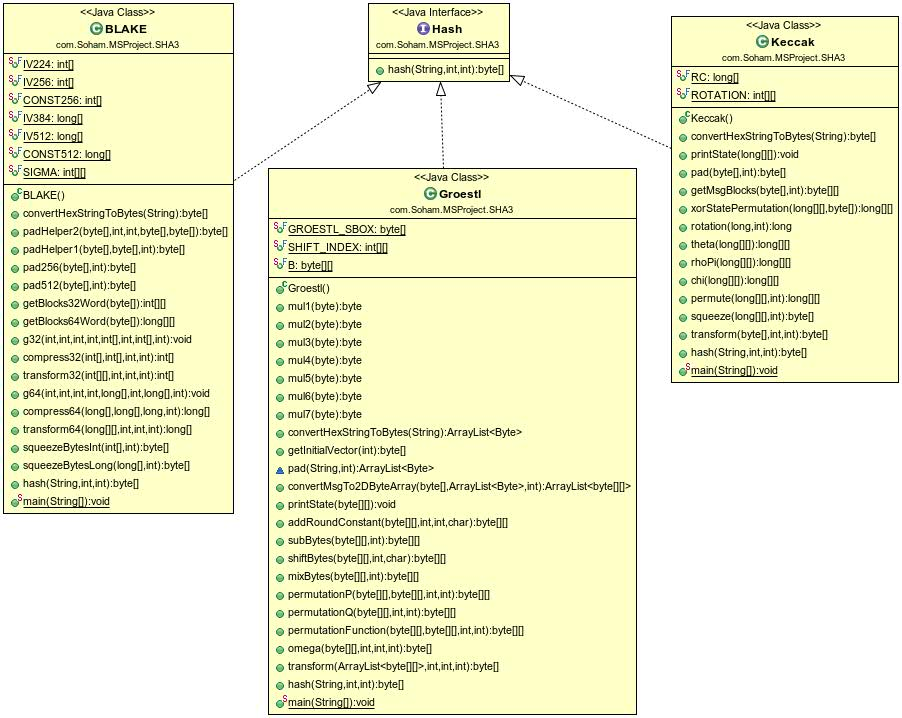
\includegraphics[width=7in]{SHA3classes.jpg}
  \end{center}
  \caption{Class diagram of the classes for the 3 hash functions implemented.}
  \label{fig:UMLSHA3classes}
\end{figure}

\begin{figure}
  \begin{center}
    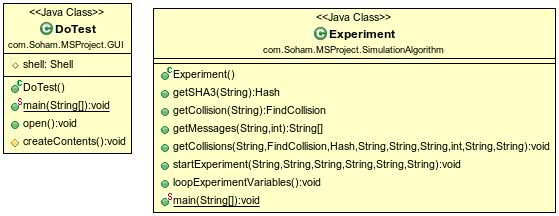
\includegraphics[width=5.65in]{ExperimentGUIClass.jpg}
  \end{center}
  \caption{Class diagram of the GUI class and the initiation of experiment.}
  \label{fig:UMLExperimentGUIClass}
\end{figure}

\begin{figure}
  \begin{center}
    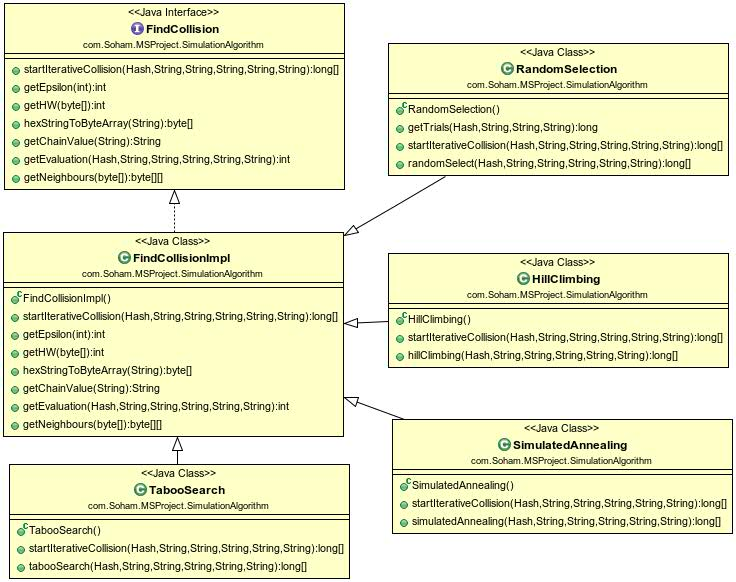
\includegraphics[width=7in]{FindCollisionClasses.jpg}
  \end{center}
  \caption{Class diagram of the classes for finding collisions.}
  \label{fig:UMLCollisionFindingClasses}
\end{figure}

\begin{figure}
  \begin{center}
    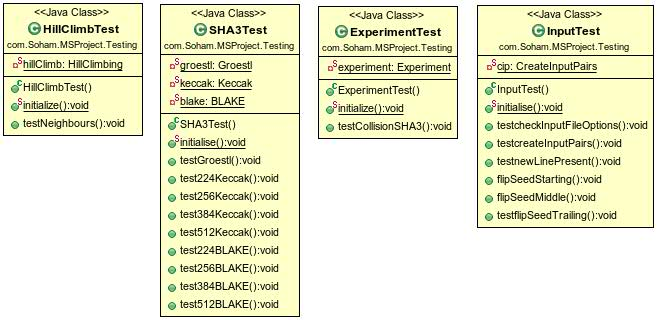
\includegraphics[width=6.75in]{testingcode.jpg}
  \end{center}
  \caption{Class diagram of the classes used for testing, using JUnit4.}
  \label{fig:UMLJUnitTestClasses}
\end{figure}
